\chapter{Projeto Conceitual do Produto}

\label{projeto}

\section{Características gerais}

%\textcolor{red}{Descrever produto de forma geral. Apresentar itens teóricos sobre o projeto a serem aprofundados ou detalhados oportunamente.}

%\textcolor{red}{Apresentar e explicar a Estrutura Analítica do Projeto (EAP), tomando cuidado com a legibilidade da imagem. Se necessário, coloque a EAP dentro do comando ``\textsf{\textbackslash begin\{landscape\} \textbackslash end\{landscape\}}'' para que ela seja apresentada em uma página deitada.}

O Micromouse é um robô móvel autônomo desenvolvido para mapear e resolver labirintos desconhecidos em matrizes de $4\times4$, $8\times8$ e $16\times16$ células, com o objetivo de alcançar a região central no menor tempo possível. O produto integra tecnologias multidisciplinares, unindo uma estrutura física compacta a um ecossistema de software para monitoramento em tempo real.

O hardware é baseado no microcontrolador ESP32, utilizando sensores laser Time-of-Flight (ToF) para detecção de obstáculos e motores N20 com encoders para odometria. O sistema de software provê a observabilidade através de um dashboard web que exibe dados de telemetria, como trajeto, velocidade e consumo de bateria via Wi-Fi.

Os itens teóricos fundamentais para o sucesso do projeto, que serão detalhados oportunamente, compreendem:

\begin{itemize}
    \item \textbf{Dinâmica e Estabilidade}: Cálculos de torque, potência e análise das condições de não-tombamento para garantir manobras seguras.
    \item \textbf{Gestão Energética}: Dimensionamento de baterias Li-Ion e eficiência de conversores DC-DC Buck para autonomia operacional.
    \item \textbf{Algoritmos de Navegação}: Aplicação de lógica Flood Fill para resolução de caminho e estratégias de exploração como DFS ou Tremaux.
    \item \textbf{Arquitetura de Sistemas}: Uso do FreeRTOS para processamento dual-core paralelo entre controle e telemetria.
\end{itemize}

\subsection{Estrutura Analítica do Projeto}

A Estrutura Analítica do Projeto (EAP) apresentada nesta seção é uma decomposição hierárquica orientada a entregas, porém, com foco no produto, organizada para facilitar o gerenciamento e o controle do escopo. O produto, e consequentemente o projeto, está dividido em cinco macroáreas principais:

\begin{itemize}
    \item \textbf{Estruturas (Laranja):} Abrange o desenvolvimento da estrutura física do robô e do labirinto de teste, incluindo base, chassi, fixações, rodas e organização mecânica.

    \item \textbf{Energia (Rosa):} Envolve a definição e integração do sistema de alimentação, incluindo bateria, reguladores de tensão, distribuição de energia e proteção do circuito.

    \item \textbf{Sistema de software (Verde):} Abrange o desenvolvimento da lógica de controle do robô, incluindo leitura dos sensores, controle dos motores, algoritmo de navegação e comunicação com o sistema embarcado.

    \item \textbf{Sistema eletrônico embarcado (Azul):} Envolve a integração dos componentes eletrônicos, como microcontrolador, sensores, driver dos motores, encoders e conexões elétricas do robô.

    \item \textbf{Sistema integrado (Roxo):} Abrange a integração entre estrutura, energia, eletrônica e software, incluindo montagem final, testes de funcionamento, ajustes e validação do robô no labirinto.
\end{itemize}

\begin{landscape}

\begin{figure}[p]
    \centering
    
\includegraphics[
        width=\linewidth,
        height=0.80\textheight,
        keepaspectratio
    ]{figuras/eap.jpg}
    \caption{Visualização geral da Estrutura Analítica do Projeto.}
    \label{fig:eap-geral}
\end{figure}

\end{landscape}


\begin{landscape}

\begin{figure}[p]
    \centering

    \begin{minipage}{0.48\linewidth}
        \centering
        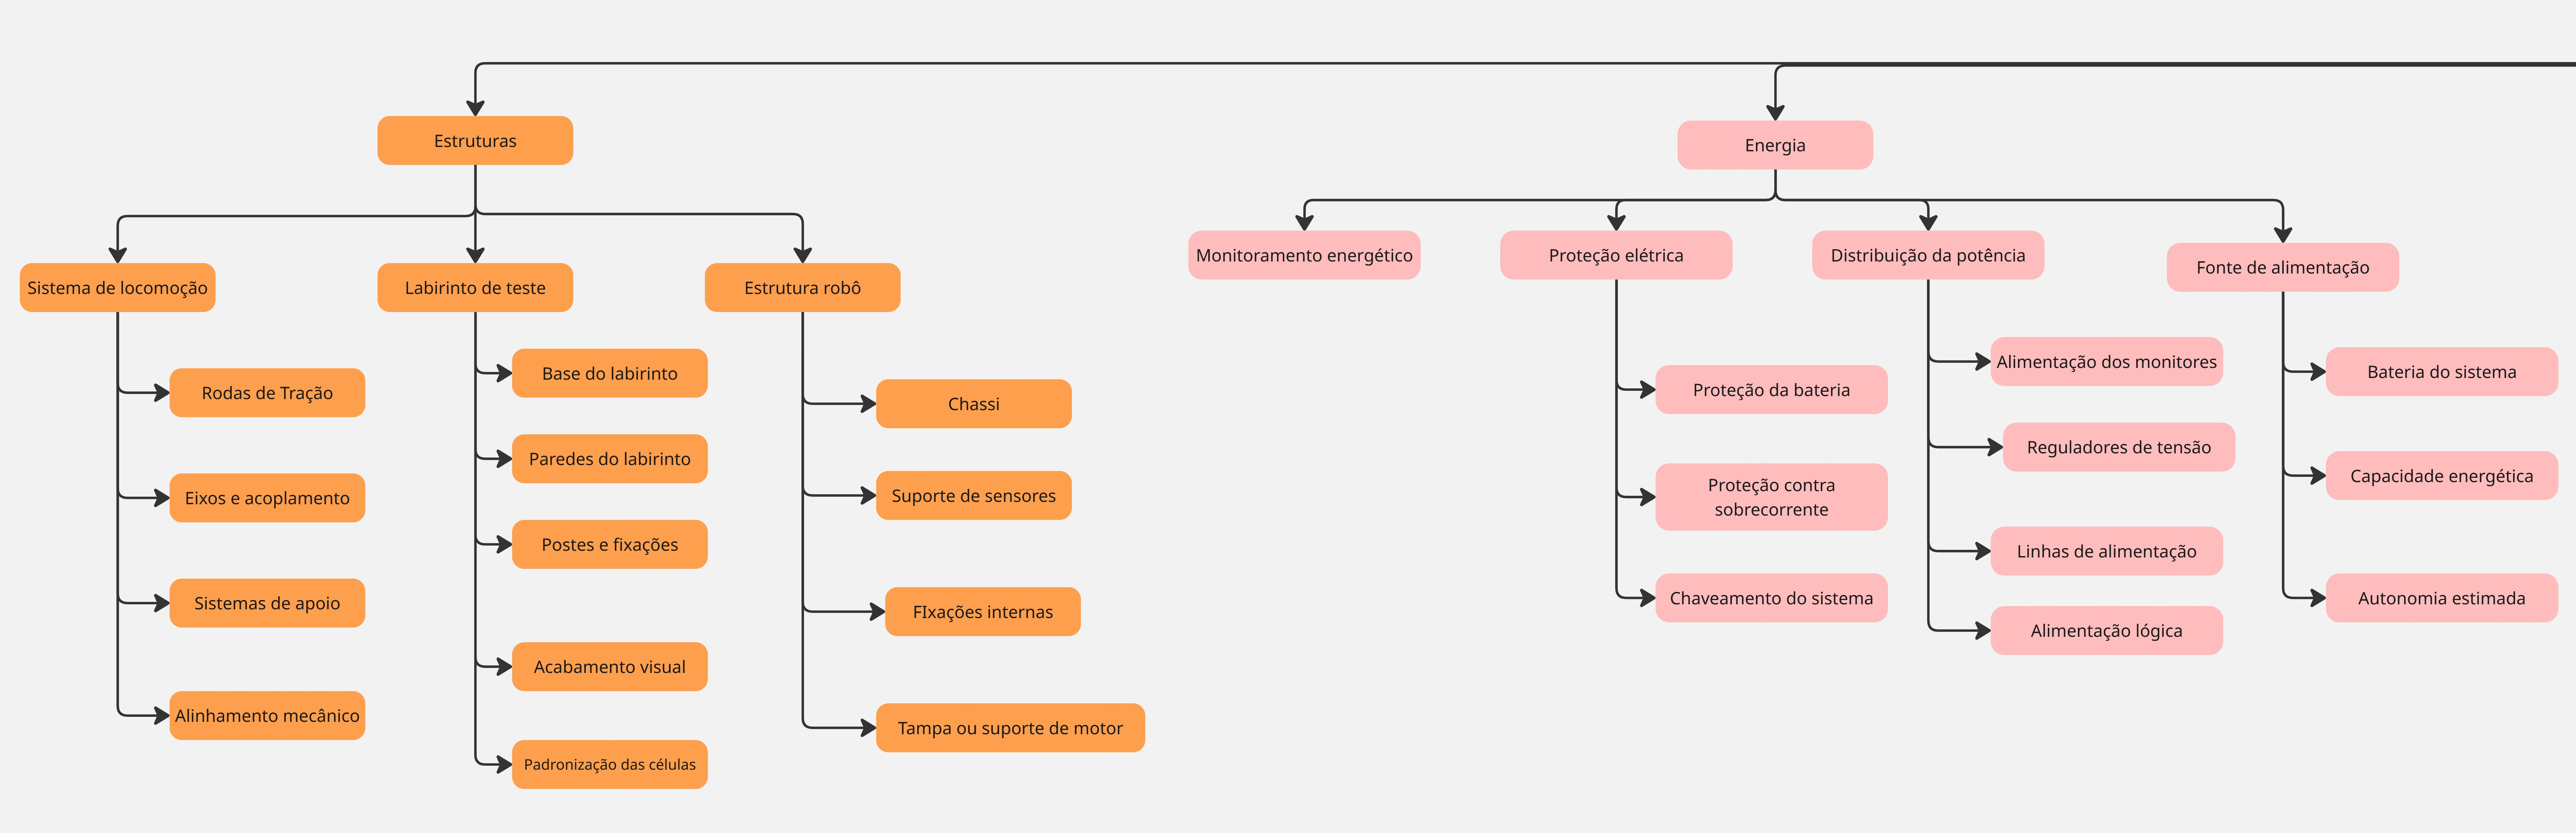
\includegraphics[
            width=\linewidth,
            height=0.72\textheight,
            keepaspectratio
        ]{figuras/eap_estruturas_energia.jpg}

        \vspace{0.2cm}
        \textbf{(a)} Primeira parte expandida do EAP.
    \end{minipage}
    \hfill
    \begin{minipage}{0.48\linewidth}
        \centering
        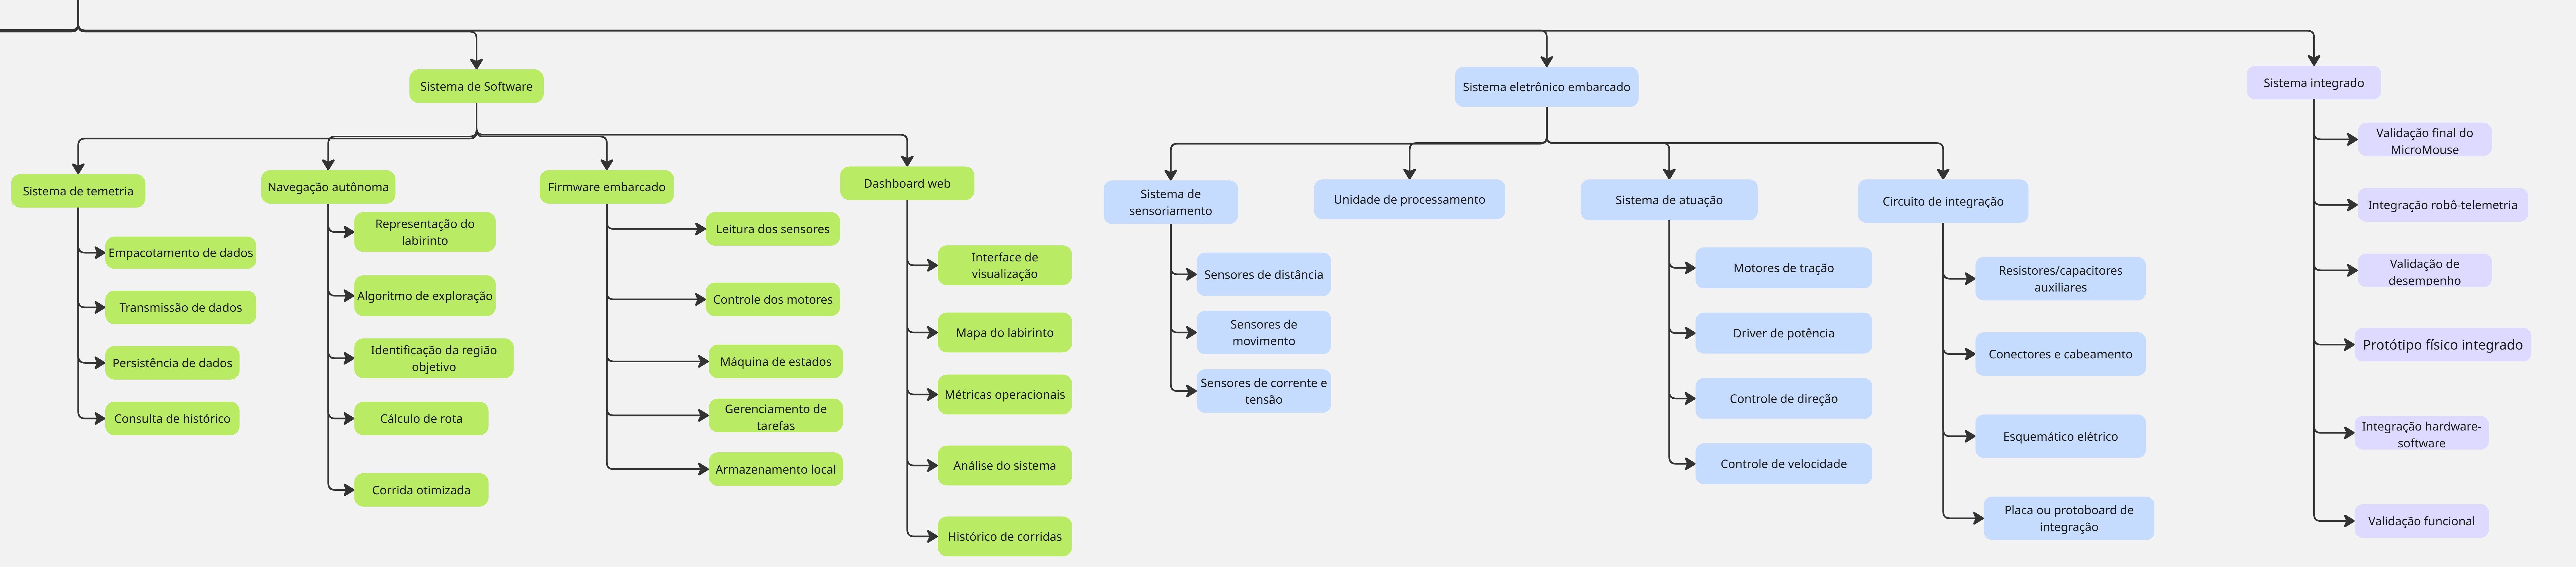
\includegraphics[
            width=\linewidth,
            height=0.72\textheight,
            keepaspectratio
        ]{figuras/eap_energia_embarcados_integrado.jpg}

        \vspace{0.2cm}
        \textbf{(b)} Segunda parte expandida do EAP.
    \end{minipage}

    \caption{Visualizações expandidas da Estrutura Analítica do Projeto.}
    \label{fig:eap-expandido}
\end{figure}

\end{landscape}

\section{Estrutura}
Esta seção descreve a síntese do projeto mecânico do Micromouse, desenvolvido sob uma perspectiva técnica e funcional. A estrutura foi projetada para equilibrar a rigidez necessária à precisão dos sensores com a leveza exigida para acelerações rápidas, respeitando rigorosamente as normas internacionais de competições de Micromouse.

Para a validação das escolhas de engenharia, este documento detalha os cálculos para determinação de dimensões e seleção dos motores, desenhos técnicos que materializam a geometria adotada e a especificação técnica dos materiais aplicados tanto no chassi quanto no labirinto de testes.

\subsection{Objetivo Geral}
Projetar e validar a estrutura física de um robô autônomo (Micromouse) e seu ambiente de simulação, garantindo uma plataforma estável, leve e de baixo custo, capaz de realizar navegação precisa e manobras de alta performance em conformidade com os padrões competitivos.

\subsubsection{Objetivos Específicos}
\begin{itemize}
    \item \textbf{Dimensionamento Geométrico:} Estabelecer as dimensões críticas do chassi (largura máxima de 110 mm) para garantir a manobrabilidade em trechos retilíneos e diagonais, evitando colisões com as paredes do labirinto.
    \item \textbf{Otimização Dinâmica:} Realizar o cálculo de torque e potência para a seleção do sistema motriz (GA12-N20), assegurando que o robô vença a inércia e mantenha a estabilidade (não-tombamento) em acelerações e frenagens bruscas.
    \item \textbf{Desenvolvimento Estrutural:} Projetar um chassi estratificado (dois níveis) que organize de forma estratégica a bateria, motores e sensores, otimizando o centro de massa e facilitando a manutenção dos componentes.
    \item \textbf{Seleção de Materiais:} Justificar o uso de materiais como PLA (impressão 3D) para o robô e MDF/EVA para o labirinto, focando na redução de peso e na qualidade da leitura dos sensores.
    \item \textbf{Padronização do Ambiente:} Construir um labirinto de testes modular que replique as condições reais de competição, permitindo a calibração fina dos algoritmos de busca e mapeamento.
\end{itemize}

\subsection{Dimensionamento Geométrico do Labirinto}

\subsubsection{Contexto e Normas do Labirinto}
O labirinto oficial da competição Micromouse é composto por células quadradas de $18{ cm} \times 18{ cm}$, medidos de centro a centro das paredes. As paredes laterais possuem $5{ cm}$ de altura e $1,2{ cm}$ de espessura. Esse padrão é adotado internacionalmente e define todas as restrições geométricas para o projeto do robô.

Considerando a espessura das paredes, o vão livre disponível para a movimentação do robô dentro de um corredor retilíneo é de:
\begin{equation}
18{ cm} - 1,2{ cm} = 16,8{ cm}
\end{equation}

Este valor é crítico porque representa o espaço real que o robô tem para efetuar o deslocamento sem tocar nas paredes laterais durante uma trajetória em linha reta. Além disso, para manobras que exigem uma rotação de $90^\circ$ ou travessia diagonal de uma célula, a geometria do labirinto impõe uma restrição mais severa: o robô não pode exceder a largura equivalente à diagonal do vão livre. O limite teórico para essa situação é:
\begin{equation}
{Largura diagonal} = 16,8{ cm} \div \sqrt{2} \approx 11,88{ cm}
\end{equation}

O projeto do chassi deve respeitar ambos os limites:
\begin{itemize}
    \item $\le 16,8{ cm}$ para trechos retos;
    \item $\le 11,88{ cm}$ para garantir operação em diagonal.
\end{itemize}

\subsubsection{Materiais e Construção do Labirinto Teste}
Para a construção do labirinto de testes, o projeto priorizou a modularidade e a fidelidade técnica às normas de competição. A estrutura baseia-se em uma malha de $4 \times 4$ células, totalizando $72{ cm}$ de lado, com vãos livres de $168{ mm}$.

Optou-se por uma base em \textbf{MDF de 6 mm}, visando planicidade e uniformidade. Para as paredes, utilizou-se \textbf{EVA de alta densidade de 12 mm}, que oferece leveza e segurança contra impactos. A montagem utiliza 25 postes removíveis ancorados à base por suportes metálicos em ``L''. As faces das paredes são revestidas com vinil branco fosco para otimizar os sensores ToF. O detalhamento geométrico completo (Figura \ref{fig:Desenho esquematoco do Labirinto de Testes}) ilustra o posicionamento dos postes e as dimesões da labirinto de testes. 

\subsection{Dimensionamento Geométrico do Chassi}

\subsubsection{Arranjo Preliminar dos Componentes}
\begin{itemize}
    \item \textbf{Bateria:} Posicionada na parte traseira para estabilizar o centro de massa.
    \item \textbf{Motores:} Localizados no centro do chassi para fornecer torque equilibrado às rodas.
    \item \textbf{Sensores:} Posicionados estrategicamente na dianteira para mapeamento e detecção de obstáculos.
\end{itemize}

\subsubsection{Desenho Esquemático}
O desenho técnico do chassi segue as larguras máximas de $160{ mm}$ (retilíneo) e $118,8{ mm}$ (diagonal). A vista explodida do Robô evidencia a hierarquia de montagem e as premissas de estabilidade dinâmica e fácil acesso à manutenção através da tampa
superior.

\subsubsection{Vistas Técnicas}
O desenho técnico do chassi (Figura \ref{fig:Draft Micromouse}) apresenta as principais dimensões e a localização de fixação dos componentes (motores, bateria e microcontrolador). As cotas estão expressas em milímetros e seguem as larguras máximas definidas anteriormente:
\begin{itemize}
    \item 160 mm para deslocamento retilíneo;
    \item 118,8 mm para manobras diagonais.
\end{itemize}

\subsubsection{Vista Explodida e Arranjo de Componentes}
A vista explodida do robô (Figura \ref{fig:Draft Micromouse explodido}) evidencia a disposição espacial dos 13 subsistemas principais, permitindo visualizar a hierarquia de montagem e a integração entre as partes mecânicas e eletrônicas.

\begin{table}[htbp]
\centering
\caption{Lista de Peças}
\label{tab:pecas_micromouse}
\begin{tabular}{@{}clc@{}}
\toprule
\textbf{Número} & \textbf{Nome} & \textbf{Quantidade} \\ \midrule
1 & Chassis & 1 \\
2 & Motor & 2 \\
3 & Bateria & 1 \\
4 & Microcontrolador & 1 \\
5 & Lateral & 2 \\
6 & Roda & 4 \\
7 & Engrenagem & 2 \\
8 & Protoboard 400 pinos & 1 \\
9 & Protoboard 170 pinos & 2 \\
10 & Tampa & 1 \\
11 & Sensor Laser VL53l0x & 3 \\
12 & Conversor DC-DC & 2 \\
13 & Driver para motor & 1 \\ \bottomrule
\end{tabular}
\end{table}

O arranjo foi projetado seguindo as seguintes premissas:

\begin{itemize}
    \item \textbf{Estabilidade Dinâmica:} A bateria (item 3) e os motores (item 2) estão fixados no chassi inferior (item 1), mantendo o centro de massa o mais próximo possível do solo e garantindo estabilidade em curvas.
    \item \textbf{Acesso à manutenção:} A tampa (item 10) permite a separação funcional dos componentes. Aqueles que não necessitam de acesso constante (motores, bateria) são alocados no chassi (item 1). Os elementos que exigem intervenção constante para depuração e calibração ficam acessíveis no plano superior. Além de prover proteção passiva, a tampa integra aberturas para o gerenciamento de cabos.
    \item \textbf{Interface de sensoriamento:} Os suportes dos sensores laser (item 11) foram posicionados nas extremidades da base, assegurando que o envelope de leitura não sofra interferência das rodas ou da tampa superior.
\end{itemize}

\subsubsection{Visão Isométrica}
A perspectiva isométrica do Micromouse (Figura \ref{fig:iso do micromouse}) consolida o design tridimensional, permitindo a visualização do robô em seu estado final de montagem.

\begin{itemize}
    \item \textbf{Validação volumétrica:} Demonstra a capacidade do conjunto e seu respeito às dimensões do labirinto.
\end{itemize}

\subsection{Dimensionamento dos Motores}

Pela Segunda Lei de Newton, a força trativa ($F_t$) deve superar a resistência ao rolamento ($F_{rr}$) para imprimir uma aceleração constante ($a$):

\begin{equation}
    C_{rr} = \frac{b}{R} \quad ; \quad F_{rr} = C_{rr} \cdot m \cdot g
\end{equation}

Onde $b$ é o coeficiente de atrito de rolamento, $R$ o raio da roda, $m$ a massa ($m \le 0,250{kg}$) e $g$ a aceleração da gravidade. A força trativa total é dada por:

\begin{equation}
    F_t = m \cdot (a + C_{rr} \cdot g)
\end{equation}

O torque mínimo ($T_{\min}$) e o torque de projeto com margem ($T_{{proj}}$) são definidos, respectivamente, pelas equações \ref{eq:torque_min} e \ref{eq:torque_projeto}:

\begin{equation}
    T_{\min} = F_t \cdot R
    \label{eq:torque_min}
\end{equation}

\begin{equation}
    T_{{proj}} = T_{\min} \cdot 1,3
    \label{eq:torque_projeto}
\end{equation}

\subsubsection{Desenvolvimento Matemático}

Adotou-se $b = 1,5{mm}$ (silicone sobre madeira pintada) e $R = 22,5{mm}$. Os cálculos seguem no Sistema Internacional (SI):

\begin{equation}
    F_{rr} = \left(\frac{1,5}{22,5}\right) \cdot 0,25 \cdot 9,81 = 0,1635{N}
\end{equation}

Logo, a força trativa para uma aceleração de $1{m/s}^2$ é:

\begin{equation}
    F_t = 0,25 \cdot 1 + 0,1635 = 0,4135{N}
\end{equation}

O torque mínimo total e o torque por motor (dividido por 2 com margem de 30\%) resultam em:

\begin{equation}
    T_{\min} \approx 9,31{N.mm} \Longrightarrow T_{\min\_{motor\_proj}} = \frac{9,31 \cdot 1,3}{2} = 6,0515{N.mm}
\end{equation}

\subsubsection{Conclusão e Validação}

Comparando os valores calculados com o \textit{datasheet} do motor \textbf{GA12-N20-S0310D-E}:

\begin{table}[htbp]
    \centering
    \caption{Validação do torque do motor GA12-N20}
    \label{tab:validacao-motor}
    \small
    \renewcommand{\arraystretch}{1.5}
    \begin{tabular}{|l|c|c|c|}
        \hline
        \textbf{Parâmetro} & \textbf{Valor Datasheet} & \textbf{Valor (N.mm)} & \textbf{Status} \\ \hline
        Torque Nominal     & 2,9~kg.mm                & 28,44~N.mm            & Validado ($> 6,05$) \\ \hline
        Torque de Estol    & 17~kg.mm                 & 166,71~N.mm           & Validado ($> 6,05$) \\ \hline
    \end{tabular}
\end{table}

\subsection{Condições de Não-Tombamento}

\subsubsection{Objetivo e Fundamentação Teórica}

O objetivo desta análise é determinar a altura máxima permitida para o Centro de Gravidade (CG), de forma a garantir que o veículo permaneça estável e não capote durante frenagens bruscas.

Na iminência de tombamento, a força Normal no eixo traseiro torna-se nula. A estabilidade é mantida enquanto o torque restaurador for superior ao torque de tombamento:

\begin{itemize}
    \item \textbf{Torque Restaurador:} Gerado pela componente vertical do peso.
    \item \textbf{Torque de Tombamento:} Gerado pela força de inércia resultante da desaceleração.
\end{itemize}

\subsubsection{Desenvolvimento Matemático}

A condição de estabilidade em relação ao eixo frontal é definida por:

\begin{equation}
    \tau_{{restaurador}} \geq \tau_{{tombamento}}\Longrightarrow P \cdot x \geq F \cdot h_{{máx}}
\end{equation}

Considerando que a força de desaceleração máxima é limitada pelo atrito estático ($\mu_e$), temos $F = P \cdot \mu_e$. Assim:

\begin{equation}
    P \cdot x \geq (P \cdot \mu_e) \cdot h_{máx}\Longrightarrow h_{{máx}} \le \frac{x}{\mu_e}
\end{equation}

Para uma distribuição de massa ideal, onde o CG está no centro geométrico ($x = L/2$):

\begin{equation}
    h_{{máx}}\le\frac{L}{2\cdot\mu_e}
\end{equation}

Dados os parâmetros do projeto:
\begin{itemize}
    \item $\mu_e = 0,7$
    \item $L = 0,1225~{m}$
\end{itemize}

\begin{equation}
    h_{máx}\le \frac{0,1225}{2 \cdot 0,7} \approx 0,0875{m} \Longrightarrow h_{máx} \le 8,75{cm}
\end{equation}

\subsubsection{Conclusão}
A análise do projeto mecânico confirma que o robô está tecnicamente apto para a competição. Com largura de $110{ mm}$ e centro de gravidade otimizado, o Micromouse garante agilidade sem risco de colisões ou tombamentos. O sistema motriz validado e o labirinto de testes fiel às normas consolidam uma base sólida para a integração final dos algoritmos de navegação autônoma.

\section{Análise de consumo energético}

Esta seção apresenta o dimensionamento energético do sistema embarcado do MicroMouse, considerando os componentes eletrônicos utilizados, o tempo estimado de operação e a escolha da fonte de alimentação. O objetivo é estimar o consumo total do sistema e justificar a escolha da bateria utilizada no projeto.

\subsection{Parâmetros considerados}

Para o dimensionamento energético, considerou-se o uso do sistema durante \textbf{1080 segundo (s)}, o equivalente a 18 minutos. Esse tempo foi definido levando em conta 9 tentativas, por ser o máximo de tentativas possíveis durante a prova, e a duração de 2 minutos por tentativa.

Também foi adotada uma margem de segurança de 30\% sobre o consumo total estimado, a fim de reduzir o risco de subdimensionamento da bateria e garantir maior confiabilidade ao sistema.

\subsection{Relação dos componentes}

A Tabela~\ref{tab:componentes-energia} apresenta os principais componentes eletrônicos considerados no cálculo energético do sistema.

\begin{table}[htbp]
\centering
\caption{Componentes considerados no dimensionamento energético}
\label{tab:componentes-energia}
\small
\setlength{\tabcolsep}{4pt}
\renewcommand{\arraystretch}{1.2}
\begin{tabularx}{\textwidth}{|>{\raggedright\arraybackslash}X|c|c|c|c|}
\hline
\textbf{Componente} & \textbf{Qtd.} & \textbf{Tensão (V)} & \textbf{Corrente (A)} & \textbf{Tempo (s)} \\ \hline

ESP WROOM-32 / ESP32 DevKit V1 
& 1 & 5 & 0,08 a 0,5 & 1080 \\ \hline

Motor GA-12 N20 DC com encoder 
& 2 & 6 & 0,08 a 1,6 & 1080 \\ \hline

Sensor ToF VL53L0X 
& 3 & 2,8 & 0,02 & 1080 \\ \hline

Sensor INA219 
& 1 & 3,3 & 0,001 & 1080 \\ \hline

\end{tabularx}
\end{table}

A Ponte H TB6612FNG não foi contabilizada diretamente no dimensionamento energético, pois atua como intermediária no acionamento dos motores. Dessa forma, o consumo dos motores GA-12 N20 já representa a maior parte da corrente que passa por ela. O consumo próprio da lógica interna da TB6612FNG é muito pequeno em relação ao consumo total do sistema e, por isso, foi considerado desprezível para este cálculo.

\subsection{Cálculo da energia consumida por componente}

A energia consumida por cada componente foi calculada por meio da 
Equação~\ref{eq:energia}, utilizando os parâmetros de tensão, corrente 
e tempo listados na Tabela~\ref{tab:componentes-energia}.

\begin{equation}
E_{J} = V \cdot I \cdot t
\label{eq:energia}
\end{equation}

No qual $E$ representa a energia consumida em joules (J), $V$ é a tensão 
de operação em volts (V), $I$ é a corrente elétrica em amperes (A) e 
$t$ é o tempo de uso em segundos (s). Para os componentes com faixa de 
corrente, adotou-se o valor máximo, representando o pior caso de consumo.

Para converter o resultado de joules para watt-hora(Wh), utilizou-se a 
relação da Equação~\ref{eq:conversao_j_wh}:

\begin{equation}
E_{Wh} = \frac{E_{J}}{3600}
\label{eq:conversao_j_wh}
\end{equation}

A Tabela~\ref{tab:consumo-individual} apresenta, para cada componente, 
a aplicação da Equação~\ref{eq:energia} com os parâmetros da 
Tabela~\ref{tab:componentes-energia}, o resultado em joules,
conversão para watt-hora pela Equação~\ref{eq:conversao_j_wh} e o resultado em watt-hora.

\begin{table}[h]
\centering
\caption{Consumo energético individual dos componentes em 18 minutos}
\label{tab:consumo-individual}
\resizebox{\linewidth}{!}{
\begin{tabular}{|l|l|c|c|c|}
\hline
\textbf{Componente} & \textbf{Equação \ref{eq:energia}} & \textbf{Energia (J)} & \textbf{Equação \ref{eq:conversao_j_wh}} & \textbf{Energia (Wh)} \\ \hline
ESP32 DevKit V1 & $E_{J} = 5 \cdot 0{,}5 \cdot 1080$ & 2700 &  $E_{Wh} = 2070 \div 3600 $ & 0,75 \\ \hline
Motor GA-12 N20 & $E_{J} = 6 \cdot 1{,}6 \cdot 1080$ & 10368 & $E_{Wh} = 10368 \div 3600 $  & 2,88 \\ \hline
Sensor ToF VL53L0X & $E_{J} = 2{,}8 \cdot 0{,}02 \cdot 1080$ & 60,48 & $E_{Wh} = 60,48 \div 3600 $ & 0,0168 \\ \hline
Sensor INA219 & $E_{J} = 3{,}3 \cdot 0{,}001 \cdot 1080$ & 3,564 & $E_{Wh} = 3,564 \div 3600 $ & 0,001 \\ \hline
\end{tabular}
}
\end{table}

\subsection{Estimativa do consumo total de energia}

Para obter o consumo total, o consumo individual de cada componente foi multiplicado pela respectiva quantidade utilizada no sistema, conforme apresentado na Tabela~\ref{tab:consumo-total}.

\begin{table}[htbp]
\centering
\caption{Consumo total estimado do sistema}
\label{tab:consumo-total}
\small
\setlength{\tabcolsep}{4pt}
\renewcommand{\arraystretch}{1.2}
\begin{tabularx}{\textwidth}{|>{\raggedright\arraybackslash}X|c|c|c|}
\hline
\textbf{Componente} 
& \textbf{Qtd.} 
& \shortstack{\textbf{Consumo}\\\textbf{individual}\\\textbf{(Wh)}} 
& \shortstack{\textbf{Consumo}\\\textbf{total}\\\textbf{(Wh)}} \\ \hline

ESP32 DevKit V1 
& 1 
& 0,75 
& 0,75 \\ \hline

Motor GA-12 N20 DC com encoder 
& 2 
& 2,88 
& 5,76 \\ \hline

Sensor ToF VL53L0X 
& 3 
& 0,0168 
& 0,0504 \\ \hline

Sensor INA219 
& 1 
& 0,001 
& 0,001 \\ \hline

\textbf{Total final} 
& -- 
& -- 
& \textbf{6,5614} \\ \hline

\end{tabularx}
\end{table}

Portanto, o consumo total estimado para 18 minutos de operação é de aproximadamente:

\begin{equation}
E_{total} \approx 6{,}56\,Wh
\end{equation}

Aplicando uma margem de segurança de 30\%:

\begin{equation}
E_{folga} = 6{,}56 \cdot 1{,}30 \approx 8{,}53\,Wh
\end{equation}


Assim, a fonte de alimentação deve ser dimensionada para fornecer, no mínimo, aproximadamente \textbf{$8{,}53\,Wh$}.

\subsection{Escolha da fonte de alimentação}

Para escolher a fonte de alimentação do sistema, foi utilizada a relação entre energia, tensão e capacidade, apresentada na Equação~\ref{eq:capacidade}.

\begin{equation}
Capacidade = \frac{E}{V}
\label{eq:capacidade}
\end{equation}

Onde a capacidade é dada em ampère-hora (Ah), $E$ representa a energia necessária em watt-hora (Wh) e $V$ representa a tensão da bateria em volts (V).

Considerando a energia com folga de $8{,}53\,Wh$, foram analisadas duas possibilidades de tensão: $7{,}4\,V$ e $12\,V$.

\begin{table}[htbp]
\centering
\caption{Capacidade mínima sem considerar a profundidade de descarga}
\label{tab:capacidade-minima}
\begin{tabular}{|c|c|c|}
\hline
\textbf{Tensão da bateria} & \textbf{Cálculo} & \textbf{Capacidade mínima} \\ \hline
$7{,}4\,V$ & $8{,}53 \div 7{,}4$ & $1{,}16\,Ah$ \\ \hline
$12\,V$ & $8{,}53 \div 12$ & $0{,}71\,Ah$ \\ \hline
\end{tabular}
\end{table}

Ao dimensionar a bateria, recomenda-se considerar apenas parte da capacidade nominal como capacidade útil, evitando descargas excessivas e preservando a vida útil da bateria. Neste projeto, foram adotados os seguintes valores: \textbf{80\% de capacidade útil para baterias Li-Ion e 70\% de capacidade útil para baterias LiPo}.

\begin{table}[htbp]
\centering
\caption{Capacidade mínima corrigida considerando a capacidade útil da bateria}
\label{tab:capacidade-corrigida}
\begin{tabular}{|l|c|c|}
\hline
\textbf{Tipo de bateria} & \textbf{7,4 V} & \textbf{12 V} \\ \hline
Li-Ion & $1{,}16 / 0{,}8 \approx 1{,}46\,Ah$ & $0{,}71 / 0{,}8 \approx 0{,}89\,Ah$ \\ \hline
LiPo & $1{,}16 / 0{,}7 \approx 1{,}66\,Ah$ & $0{,}71 / 0{,}7 \approx 1{,}01\,Ah$ \\ \hline
\end{tabular}
\end{table}

\subsection{Fonte de alimentação escolhida}

A fonte de alimentação escolhida foi uma \textbf{bateria Li-Ion de $7{,}4\,V$ e $2500\,mAh$ com BMS}, considerando o custo-benefício em relação às baterias LiPo e a compatibilidade com o sistema embarcado.

Como a capacidade mínima calculada para uma bateria Li-Ion de $7{,}4\,V$ foi de aproximadamente $1{,}46\,Ah$, a bateria escolhida, com $2{,}5\,Ah$, atende ao requisito de autonomia com margem adicional de segurança.

A energia nominal da bateria escolhida é dada por:

\begin{equation}
E = V \cdot Ah
\end{equation}

\begin{equation}
E = 7{,}4 \cdot 2{,}5 = 18{,}5\,Wh
\end{equation}


Considerando o uso recomendado de 80\% da capacidade para baterias Li-Ion:

\begin{equation}
E_{util} = 18{,}5 \cdot 0{,}8 = 14{,}8\,Wh
\end{equation}


Como a energia útil disponível é maior do que a energia necessária com folga, sendo \textbf{14{,}8\,Wh > 8{,}53\,Wh}, conclui-se que a bateria escolhida \textbf{atende ao consumo estimado do sistema para 18 minutos de operação}.


\subsection{Estimativa de autonomia}

Considerando que o sistema consome aproximadamente $6{,}56\,Wh$ em 18 minutos, o consumo médio em potência é:

\begin{equation}
P_{media} = \frac{6{,}56\,Wh}{0{,}3\,h} \approx 21{,}87\,W
\end{equation}

Usando a energia útil da bateria escolhida:

\begin{equation}
Autonomia = \frac{14{,}8\,Wh}{21{,}87\,W} \approx 0{,}67\,h \approx 40\,min
\end{equation}


Portanto, a bateria escolhida possui autonomia estimada de aproximadamente \textbf{40 minutos}, considerando o consumo calculado. Caso seja considerada a margem de segurança de 30\% como consumo adicional, a autonomia estimada fica próxima de 31 minutos, ainda superior aos 18 minutos exigidos. Cabe frizar que a bateria escolhida pelo grupo é \textbf{recarregável}, o que possibilita sua reutilização em diferentes testes e ciclos de operação, a fim de reduzir a necessidade de substituição frequente e torna a solução mais prática e econômica para o projeto.

\subsection{Planejamento do circuito de alimentação}

A tensão de \textbf{$7{,}4\,V$} foi escolhida por ser adequada para o sistema embarcado, e serão utilizados de \textit{\textbf{bucks}} para formar reguladores de tensão nas entradas necessárias, protegendo a ESP32 e a ponte H contra tensões acima do limite permitido.


\subsection{Proteção da bateria com BMS}

O BMS, sigla para \textit{Battery Management System}, ou sistema de gerenciamento de bateria, é responsável por proteger as células contra condições inseguras de operação. Esse circuito auxilia na proteção contra sobrecarga, descarga excessiva e, dependendo do modelo, sobrecorrente e curto-circuito.

Mesmo com o uso do BMS, é necessário verificar se ele suporta a corrente máxima exigida pelo sistema, principalmente durante a partida dos motores, momento em que a corrente pode ser maior do que durante o funcionamento normal.

\subsection{Monitoramento via \textit{software}}

O monitoramento energético será realizado por meio do \textit{software} embarcado a ser implementado na ESP32, utilizando o sensor INA219 para acompanhar grandezas elétricas do sistema, como tensão e corrente. A comunicação com o sensor será feita por meio do barramento $I^2C$, o que permite a coleta periódica dos dados durante a operação do carrinho.

As rotinas implementadas no \textit{firmware} terão como objetivo registrar a tensão da bateria, estimar o tempo de operação e acompanhar possíveis variações no consumo de energia. Esses dados serão enviados para a aplicação de acompanhamento do sisstema. 

Além disso, o monitoramento também contribuirá para a segurança do projeto, ao permitir identificar situações de queda excessiva de tensão na bateria. Caso a tensão atinja níveis críticos, o sistema poderá acionar alertas ou executar procedimentos de parada segura antes que ocorra descarga excessiva das células. Isso complementa ainda mais a utilização do BMS.

\subsection{Validação com testes reais}

A validação do dimensionamento energético será realizada por meio de testes práticos com o MicroMouse em operação. O objetivo desses testes será comparar o consumo estimado teoricamente com o consumo real observado durante o funcionamento do sistema.

Durante os testes, serão analisados dados como tempo de operação, queda de tensão da bateria e comportamento do consumo em diferentes condições de movimentação, como aceleração, curvas e deslocamento contínuo. Com isso, será possível validar se a bateria escolhida atende adequadamente à autonomia necessária para o projeto, como verificado no projeto conceitual.

Caso sejam observadas diferenças relevantes entre os valores teóricos e experimentais, elas serão analisadas considerando fatores como perdas nos reguladores de tensão, variações na corrente dos motores, atrito mecânico, eficiência dos conversores e oscilações naturais da carga durante a operação. Assim, será possível refinar o dimensionamento energético e ajustar o sistema, se necessário.

\subsection{Conclusão}

Com base nos cálculos realizados, o sistema apresenta consumo estimado de aproximadamente $6{,}56\,Wh$ para 18 minutos de operação. Aplicando uma margem de segurança de 30\%, a energia necessária sobe para $8{,}53\,Wh$.

A bateria escolhida, uma Li-Ion de $7,4V$ e $2500mAh$ com BMS, possui energia nominal de aproximadamente $18,5\,Wh$ e energia útil estimada de $14,8\,Wh$, considerando 80\% de capacidade utilizável. Portanto, ela atende aos requisitos energéticos do projeto com margem de segurança, além de apresentar bom custo-benefício e compatibilidade com o sistema embarcado.

\section{Descrição de \textit{software}}

Esta seção tem como objetivo descrever os artefatos gerados pela equipe de software, entre eles estão: Diagrama de atividades UML, backlog do produto e requisitos, a arquitetura de solução de software e o roteriro de testes funcionais.


\subsection{Diagrama de Atividades UML}

\begin{figure}[htpb]
    \centering
    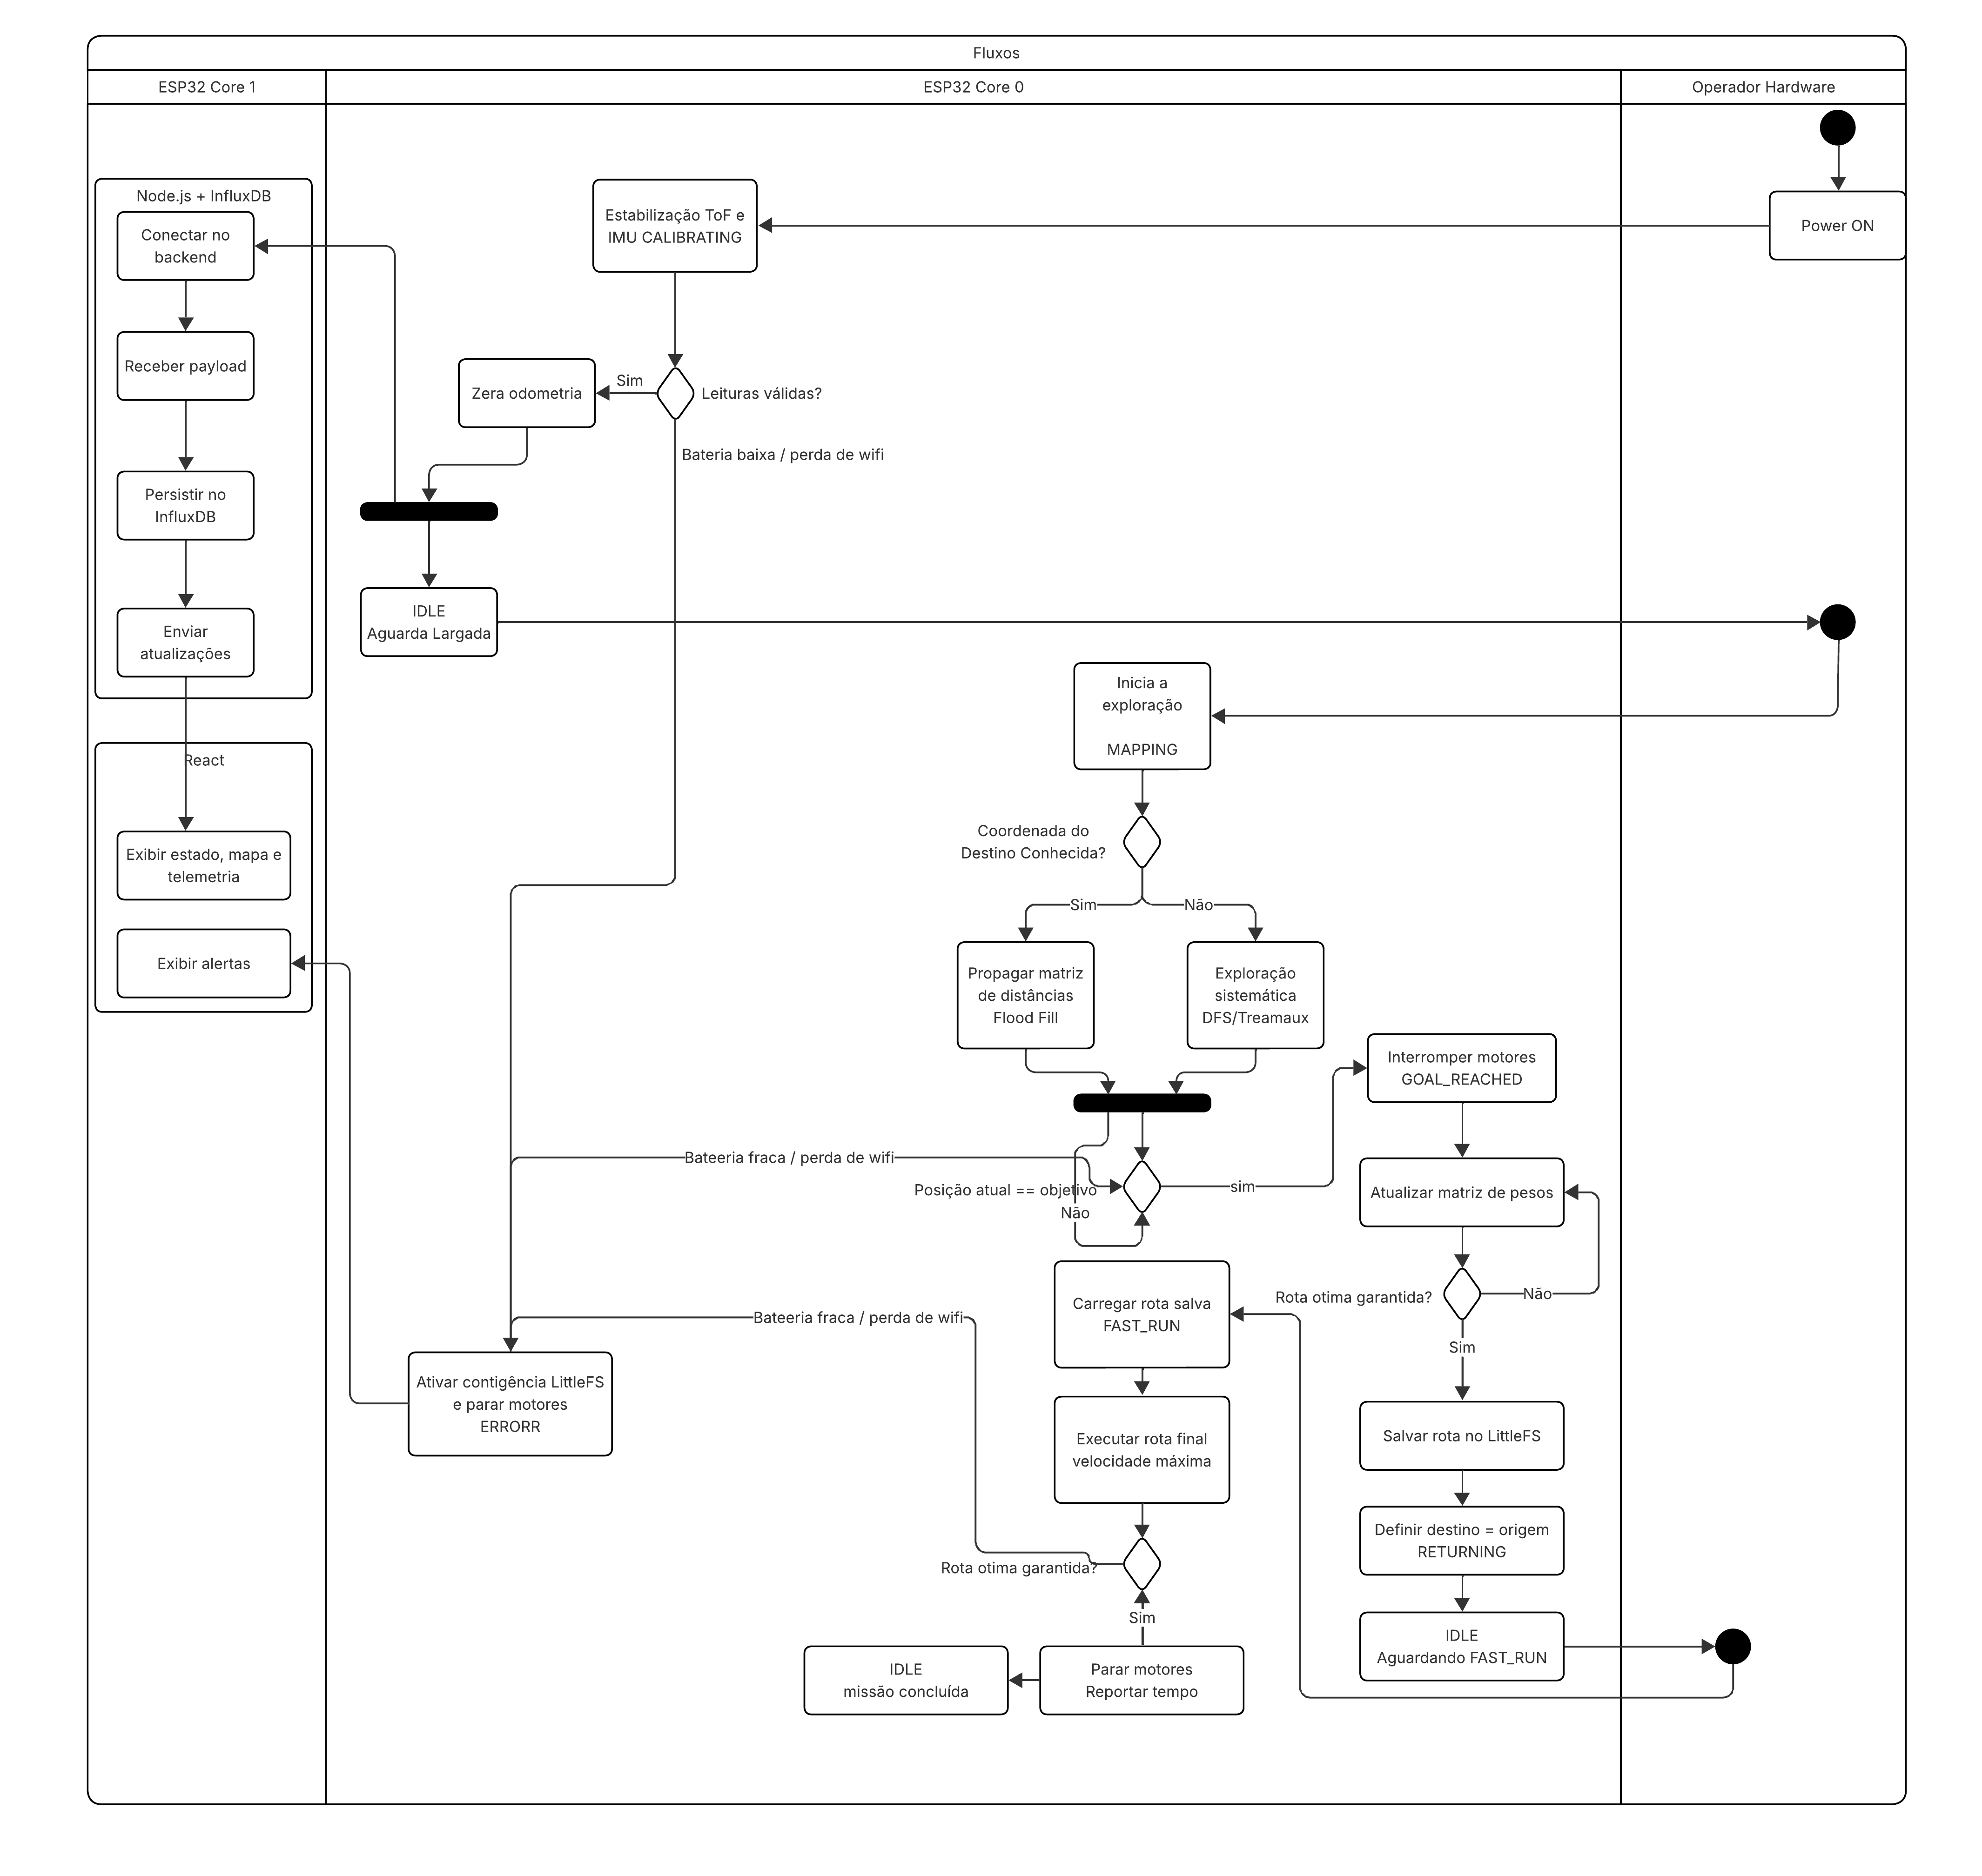
\includegraphics[width=\textwidth]{figuras/diagrama_atividades.png}
    \caption{Diagrama de Atividades UML do ecossistema Micromouse.}
    \label{fig:diagrama_atividades}
\end{figure}

O Diagrama de Atividades UML do ecossistema Micromouse é organizado em três
\textit{swimlanes} --- Operador/Hardware, ESP32 Core~0 e ESP32 Core~1 --- e
descreve o comportamento funcional do sistema ao longo de cada fase da missão.
Após o \textit{power on}, o Core~0 realiza a calibração dos sensores ToF e IMU
e, uma vez validadas as leituras, zera a odometria e avança para o estado
\texttt{IDLE}. Em seguida, um \textit{fork} dispara dois fluxos paralelos: o
Core~0 assume o controle de movimento e a FSM, enquanto o Core~1 transmite
telemetria continuamente para o \textit{backend} (Node.js + InfluxDB) e o
Dashboard em React.
Flood Fill; caso contrário, adota a exploração sistemática por DFS/Tremaux.

Na fase de exploração (\texttt{MAPPING}), o Core~0 aplica uma abordagem
híbrida: caso o destino já seja conhecido, propaga a matriz de distâncias via
O ciclo se repete até que o centro do labirinto seja atingido
(\texttt{GOAL\_REACHED}), momento em que os motores são interrompidos e a rota
ótima é calculada com base no mapa construído.

Com a rota confirmada, o destino é redefinido como a origem e o robô executa o
retorno (\texttt{RETURNING}) com controle PID, salvando o trajeto no sistema de
arquivos LittleFS. O sistema volta ao estado \texttt{IDLE} até o operador
acionar o \texttt{FAST\_RUN}, fase em que o robô percorre a rota em velocidade
máxima e reporta o tempo final. Em qualquer fase crítica, transições pontilhadas
desviam o fluxo para o estado \texttt{ERROR}, que paralisa os motores, exibe
alerta no Dashboard e aguarda o reset físico do operador.

\subsection{Backlog do Produto e Requisitos}
    \subsubsection{Backlog do Produto}
    O escopo completo da solução de \textit{software} englobando a ingestão de telemetria, o processamento de estados e a visualização no painel de controle (\textit{Dashboard})  foi especificado através de Histórias de Usuário (HUs) cobrindo a totalidade dos requisitos funcionais e operacionais. A priorização de todos os itens seguiu a classificação MoSCoW (\textit{Must have}, \textit{Should have}, \textit{Could have}, \textit{Won't have}), garantindo total rastreabilidade com os testes funcionais do sistema. A tabela contendo as histórias de usuário pode ser encontrada no backlog completo.

    \begin{figure}[htpb]
    \centering
    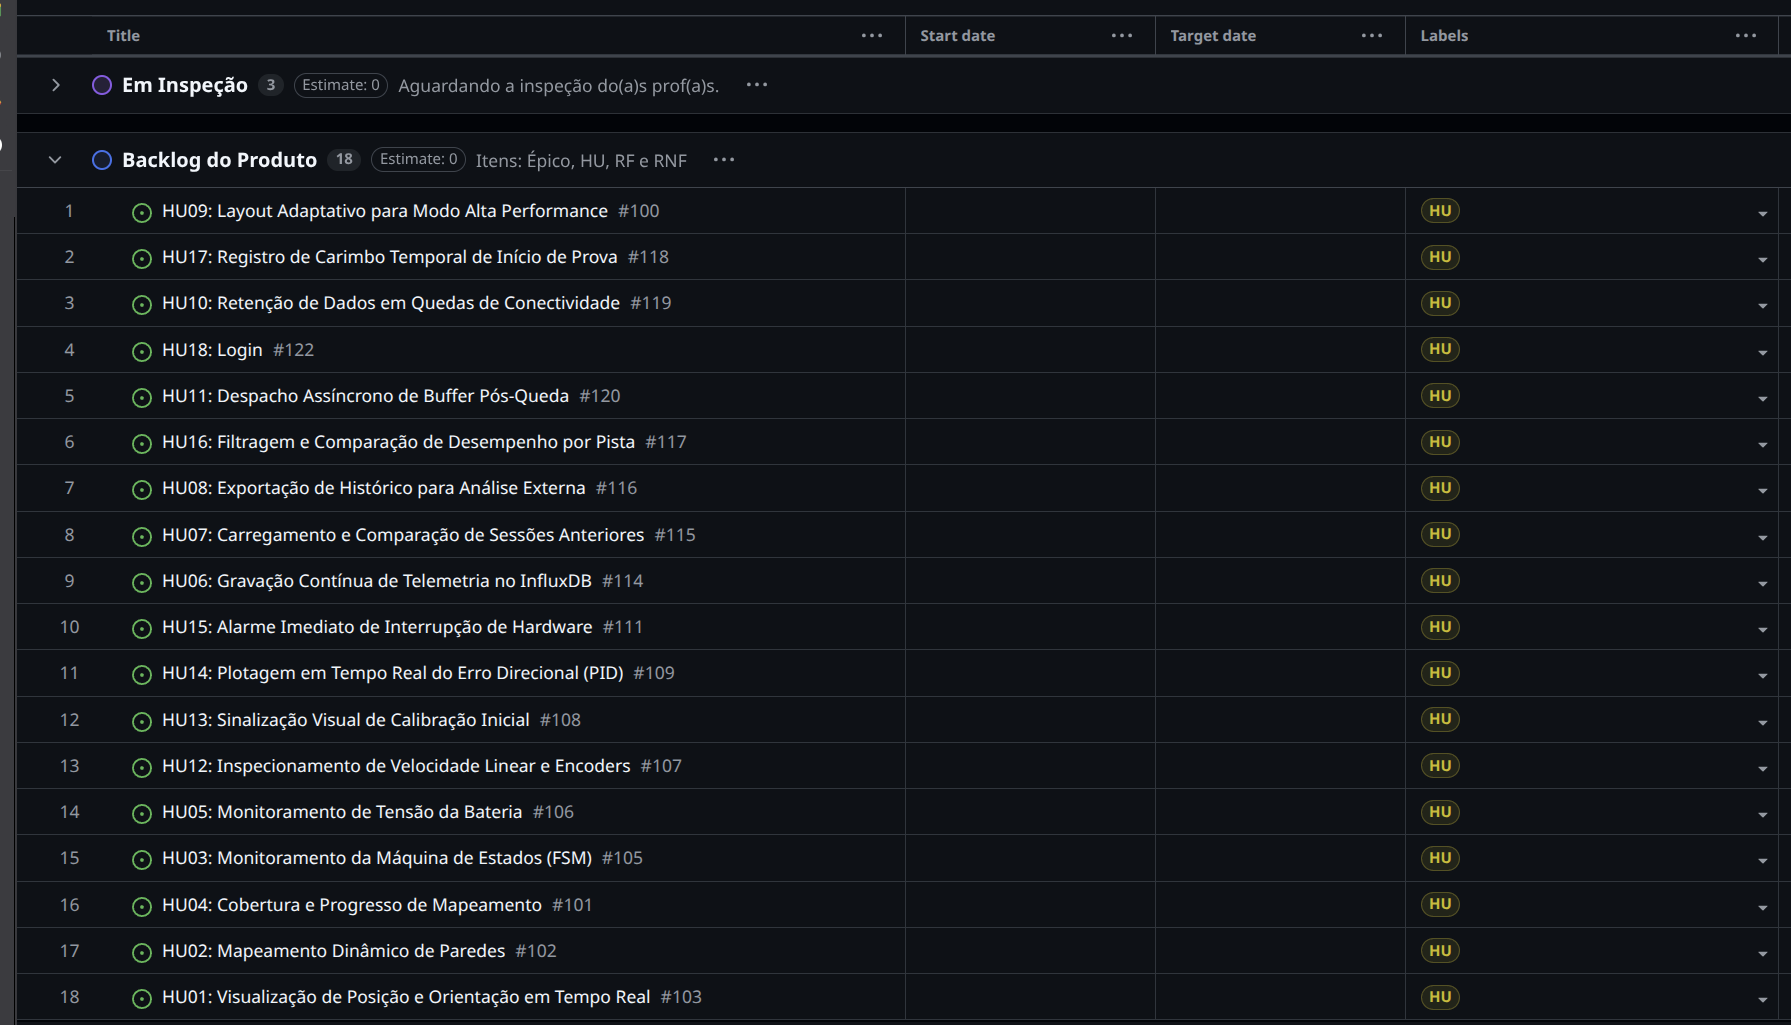
\includegraphics[width=\textwidth]{figuras/backlog_produto.png}
    \caption{Backlog do Produto}
    \label{fig:esquema-eletrico}
\end{figure}

    \subsubsection{Requisitos Funcionais e Não Funcionais}
        
    Os \textbf{Requisitos Funcionais (RF)} concentram-se na autonomia do robô: a capacidade de percepção visual do labirinto através de sensores ToF, o mapeamento interno da matriz virtual e o processamento local de algoritmos de busca de caminho. Adicionalmente, estabelecem a obrigatoriedade da transmissão de telemetria para monitoramento externo.
    
    Os \textbf{Requisitos Não Funcionais (RNF)} definem os critérios de qualidade e as restrições de contorno. Estes abrangem desde métricas de desempenho de software (como a latência máxima de transmissão) até especificações físicas rigorosas da estrutura (limites dimensionais de 10 cm de largura e massa inferior a 250 g), passando pela autonomia energética para múltiplas execuções consecutivas.
    
    Dada a natureza multidisciplinar e o rigor técnico exigido para a validação de cada item, a listagem exaustiva e a origem de cada um dos requisitos funcionais e não funcionais unificados encontram-se detalhadas no \autoref{apice:requisitos_unificados}.
                
    \subsection{Arquitetura de Solução de Software}
    
    A arquitetura do sistema é estruturada segundo as visões (4+1) do Processo Unificado (UP), segmentando a solução sob as óticas lógica, de processos, de implementação, de implantação e de dados para contemplar os requisitos multidisciplinares do Micromouse.
    
    \subsubsection{Visão Lógica}
    A visão lógica define as abstrações fundamentais, o propósito e as estratégias de navegação autônoma. O propósito do firmware embarcado é garantir a exploração e o planejamento de trajetória, enquanto a aplicação web provê a observabilidade do sistema em tempo real.

\begin{itemize}
    \item \textbf{Padrão Adotado (Arquitetura)}: O firmware adota o padrão orientado a eventos (\textit{Event-Driven Streaming}) para desacoplar a leitura de sensores da transmissão de pacotes. O Dashboard web adota o padrão baseado em Componentes com gerenciamento de estado reativo (evoluído do MVC), justificando-se pela necessidade de atualizar múltiplas métricas simultaneamente sem bloquear a interface.
    \item \textbf{Representação do Ambiente}: O labirinto é modelado como uma grade bidimensional discreta, onde cada célula armazena informações de paredes (Norte, Sul, Leste, Oeste) e estado de visitação.
    \item \textbf{Algoritmo de Navegação}: Utiliza-se o algoritmo \textit{Flood Fill} para propagar distâncias a partir da célula objetivo para as demais posições. A decisão de movimento baseia-se na seleção do vizinho acessível com o menor valor na matriz de distâncias.
    \item \textbf{Estratégia de Desempate}: Em situações de distâncias iguais, prioriza-se a manutenção da direção atual (seguindo a ordem: reta $>$ leve curva $>$ curva forte $>$ retorno) para minimizar curvas desnecessárias.
    \item \textbf{Abordagem Híbrida}: Em cenários de destino desconhecido, utiliza-se inicialmente DFS ou Tremaux para exploração sistemática, alternando para \textit{Flood Fill} assim que o objetivo é detectado.
\end{itemize}

\subsubsection{Visão de Processos}
\begin{itemize}
    \item \textbf{Processamento Dual-Core}: O microcontrolador ESP32 distribui as tarefas de forma assíncrona utilizando o FreeRTOS \cite{freertos_documentation}, o Core 0 é dedicado ao controle PID, enquanto o Core 1 gerencia a transmissão de dados via Wi-Fi, evitando interferências no movimento do robô.
    \item \textbf{Máquina de Estados Finitos (FSM)}: O firmware opera sob estados determinísticos que ditam o ciclo de vida do robô:
    \begin{itemize}
        \item \texttt{CALIBRATING}: Estabilização de sensores ToF e IMU.
        \item \texttt{IDLE}: Estado de repouso aguardando comandos.
        \item \texttt{MAPPING}: Exploração ativa e construção do mapa.
        \item \texttt{GOAL\_REACHED}: Confirmação de chegada ao centro.
        \item \texttt{RETURNING}: Retorno à base após cálculo da rota ótima.
        \item \texttt{FAST\_RUN}: Execução da rota otimizada em velocidade máxima.
        \item \texttt{ERROR}: Estado disparado por falhas críticas como bateria baixa (via INA219) ou perda de Wi-Fi.
    \end{itemize}
\end{itemize}
O diagrama da máquina de estados pode ser encontrado no \autoref{apice:maquina_de_estados}

\subsubsection{Visão de Implementação}
Descreve as linguagens e frameworks que compõem os blocos do sistema.

\begin{itemize}
    \item \textbf{Firmware (C++)}: Desenvolvido em linguagem C++ nativa, utilizando serialização MsgPack (\textit{ArduinoJson}) para otimizar o payload de telemetria, Além disso, a lógica de controle dos sensores e dos motores será organizada em \textit{tasks} do FreeRTOS \cite{freertos_documentation}.
    \item \textbf{Front-end (JavaScript/React)}: Construído em JavaScript (ES6+) utilizando a biblioteca React com Vite e Tailwind CSS. A renderização gráfica do labirinto utiliza a HTML5 Canvas API para garantir fluidez na visualização do trajeto.
    \item \textbf{Back-end (JavaScript/Node.js)}: Serviço estruturado em Node.js responsável por receber pacotes UDP e convertê-los para o protocolo de linha do InfluxDB.
\end{itemize}

\subsubsection{Visão de Implantação}
Mapeia a topologia física e a distribuição dos nós de processamento.

\begin{itemize}
    \item \textbf{Transporte de Dados}: Comunicação não-bloqueante via UDP (\textit{AsyncUDP}) com latência estimada entre 1--5 ms entre o robô e a estação base.
    \item \textbf{Fluxo de Telemetria}: ESP32 $\rightarrow$ Node.js $\rightarrow$ InfluxDB $\rightarrow$ Navegador (via WebSockets).
    \item \textbf{Resiliência}: Uso de LittleFS via SDMMC para armazenamento local contingencial em caso de falha na rede Wi-Fi.
\end{itemize}

\subsubsection{Visão de Dados (Persistência)}

Para suportar o alto volume de dados gerado em frequências de até 1 kHz, adotou-se o \textbf{InfluxDB}, um banco de dados de séries temporais (TSDB). A modelagem lógica abandona o esquema relacional tradicional em favor de um paradigma de \textit{Tags} (metadados indexados em memória) e \textit{Fields} (métricas dinâmicas gravadas em disco).

\begin{table}[htbp]
\centering
\caption{Modelagem de Dados no InfluxDB (Measurement: \texttt{log\_corrida})}
\label{tab:schema_influxdb}
\begin{tabular}{|l|l|l|}
\hline
\textbf{Tipo} & \textbf{Atributo} & \textbf{Descrição / Origem} \\ \hline
\textit{Primary Key} & \texttt{time} & Timestamp em nanossegundos \\ \hline
\textit{Tags} & \texttt{id\_labirinto} & Dimensão (ex: 16x16, 8x8) \\ \cline{2-3} 
 & \texttt{id\_corrida} & Identificador único da tentativa \\ \cline{2-3} 
 & \texttt{objetivo} & Status de conclusão (S/N) \\ \cline{2-3} 
 & \texttt{estado\_robo} & Estado da FSM embarcada \\ \hline
\textit{Fields} & \texttt{pos\_x}, \texttt{pos\_y} & Coordenadas na matriz do labirinto \\ \cline{2-3} 
 & \texttt{orientacao} & Ângulo azimutal ($\theta$) via IMU/Odometria \\ \cline{2-3} 
 & \texttt{bateria} & Tensão instantânea (Volts) via ADC1 \\ \cline{2-3} 
 & \texttt{erro\_pid} & Erro de desvio do laço de controle \\ \cline{2-3} 
 & \texttt{dist\_frontal} & Leitura do sensor ToF Frontal (mm) \\ \cline{2-3} 
 & \texttt{dist\_esq} & Leitura do sensor ToF Esquerdo (mm) \\ \cline{2-3} 
 & \texttt{dist\_dir} & Leitura do sensor ToF Direito (mm) \\ \cline{2-3} 
 & \texttt{pwm\_esq}, \texttt{pwm\_dir} & Sinal aplicado aos motores N20 \\ \cline{2-3} 
 & \texttt{velocidade\_media} & Velocidade linear (m/s) via encoders \\ \hline
\end{tabular}
\end{table}

\subsection{Roteiro de Testes Funcionais}

A validação da solução de \textit{software} fundamenta-se na execução de um roteiro de testes funcionais do tipo "caixa-preta", cujo objetivo é assegurar que todas as Histórias de Usuário descritas no \textit{backlog} operem conforme os critérios de aceitação estipulados. Este roteiro foca na integridade do fluxo de dados --- desde a captura sensorial no microcontrolador ESP32 até a renderização gráfica no \textit{Dashboard} --- e na resiliência do sistema sob condições de falha de rede ou estresse de carga.

Cada caso de teste foi estruturado para fornecer rastreabilidade total, contendo identificação única, objetivos claros, pré-condições operacionais, procedimentos passo a passo e os resultados esperados para aprovação. Essa estrutura permite que a equipe realize auditorias periódicas e garanta que novas atualizações no \textit{firmware} não causem regressões nas funcionalidades de telemetria e controle.

Devido à densidade técnica e à extensão do plano de testes, que compreende 14 cenários distintos de validação, o roteiro completo encontra-se detalhado no \autoref{apice:roteiro_testes}.

\section{Descrição de Hardware}

Esta seção apresenta a arquitetura eletrônica do sistema embarcado do Micromouse, abordando os principais componentes responsáveis pelo controle, sensoriamento, acionamento dos motores e alimentação do robô. São descritos os dispositivos utilizados no projeto, suas funções no sistema e a forma como os módulos eletrônicos se integram para garantir o funcionamento da plataforma. Além disso, são apresentados o diagrama de blocos da arquitetura, o mapeamento de comunicação entre os dispositivos e o esquemático eletrônico desenvolvido para o circuito do robô.


\subsection{Visão geral da arquitetura}


A arquitetura do sistema embarcado será representada por meio de um diagrama de blocos, com o objetivo de mostrar a organização geral do robô e a interação entre seus principais módulos. Nele são apresentados os blocos de alimentação, processamento, sensoriamento, acionamento dos motores e comunicação.


\begin{figure}[htpb]
    \centering
    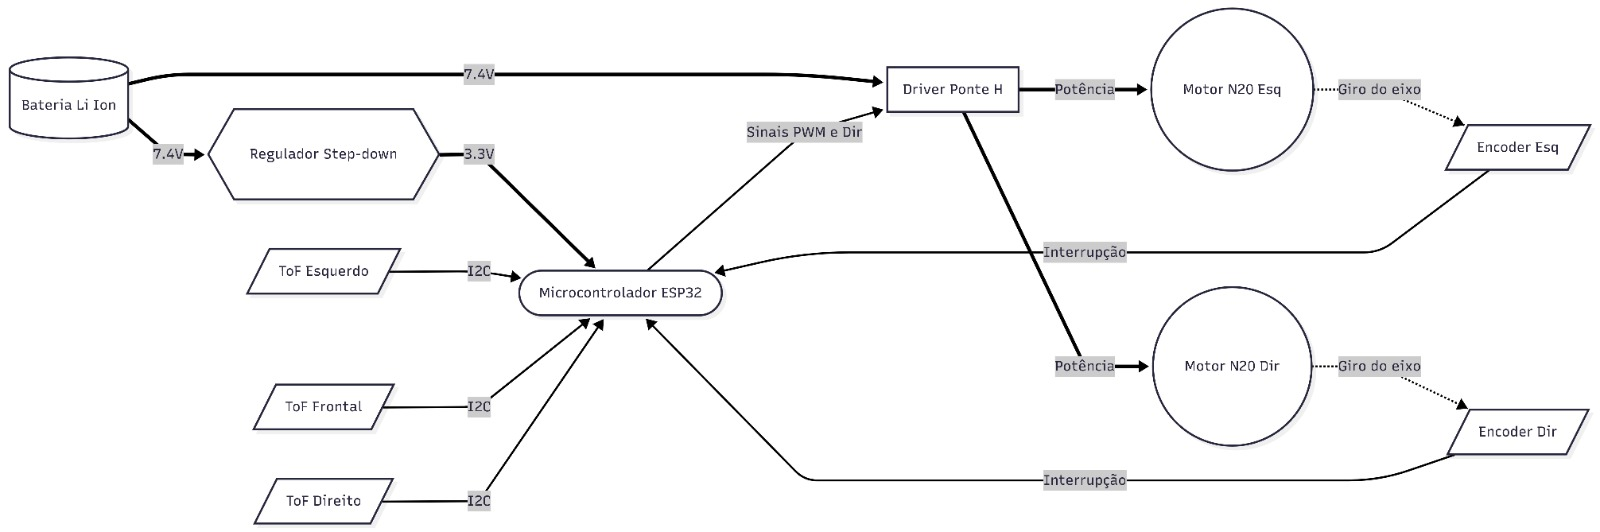
\includegraphics[width=\textwidth]{figuras/diagramaBlocos.jpeg}
    \caption{Diagrama de blocos do sistema.}
    \label{fig:diagrama-de-blocos}
\end{figure}

\subsection{Componentes eletrônicos}


\subsubsection{Microcontrolador}

O microcontrolador é o componente central do sistema embarcado do Micromouse.Eles consistem em pequenos sistemas computacionais integrados em um único chip, e contêm periféricos como memória RAM, memória Flash, interfaces de comunicação serial, conversores analógico-digitais e temporizadores \cite{chase_embarcados}.
    
Para a definição da plataforma utilizada no projeto, foi realizado um estudo comparativo entre os microcontroladores: Arduino Uno, STM32 e Raspberry Pi Pico. Após a análise, optou-se pela utilização do ESP32 DevKit WROOM devido ao seu elevado desempenho computacional, grande quantidade de periféricos integrados e suporte nativo à comunicação sem fio.

A ESP32 DevKit WROOM foi escolhida por possuir as seguintes caracteristicas: Arquitetura dual-core operando a até 240 MHz; permite dedicar um núcleo ao controle dos motores e leitura dos sensores, enquanto o outro executa os algoritmos de navegação e tomada de decisão; possui conectividade com rede Wi-fi; tem interface I²C para comunicação com sensores de distância; tem módulos PWM de alta resolução para acionamento dos motores e suporte a interrupções em múltiplos GPIOs.

%O ESP32 é um microcontrolador de alto desempenho desenvolvido para aplicações embarcadas que exigem conectividade, processamento e controle em tempo real\cite{esp32_datasheet}.Um dos principais diferenciais do ESP32 é sua arquitetura dual-core operando a até 240 MHz, permitindo a separação de tarefas críticas em diferentes núcleos de processamento. Dessa forma, é possível dedicar um núcleo ao controle dos motores e leitura dos sensores, enquanto o outro executa os algoritmos de navegação e tomada de decisão.
    
%Além disso, o ESP32 oferece periféricos fundamentais para o projeto, como interface I²C para comunicação com sensores de distância, módulos PWM de alta resolução para acionamento dos motores e suporte a interrupções em múltiplos GPIOs. Outro fator relevante é a conectividade Wi-Fi integrada, que possibilita futuras implementações de telemetria e monitoramento remoto.

    
%Dessa forma, o ESP32 apresentou a melhor relação entre desempenho, conectividade, flexibilidade e custo-benefício para atender aos requisitos do projeto.

\subsubsection{Sensores}

Os sensores de distância são componentes fundamentais para a navegação do Micromouse, uma vez que permitem a detecção de paredes e obstáculos no ambiente do labirinto sem a necessidade de contato físico. Para o projeto, foram analisadas as opçoes: sensores a laser ToF, ultrassônicos e infravermelhos.

%No contexto do projeto, os sensores de distância são responsáveis por fornecer informações em tempo real sobre a posição das paredes ao redor do robô, permitindo decisões rápidas de movimentação e correção de trajetória. Dessa forma, a escolha do tipo de sensor impacta diretamente na confiabilidade e desempenho do sistema de navegação.

Entre as tecnologias analisadas, os sensores do tipo Time-of-Flight (ToF), como o VL53L0X, destacam-se por sua alta precisão e baixo tempo de resposta, operando na ordem de milímetros. Além disso, sua medição não é significativamente afetada pela cor ou textura da superfície, o que os torna adequados para ambientes variados como labirintos. Já os sensores ultrassônicos apresentam maior alcance, porém possuem menor taxa de atualização e podem sofrer interferências devido à dispersão do sinal sonoro. Por outro lado, sensores infravermelhos são mais simples e de baixo custo, porém apresentam baixa precisão e forte dependência das condições ambientais.

Diante dessas características, o sistema do Micromouse utilizará sensores ToF como principal solução para detecção de obstáculos, posicionados nas direções frontal, esquerda e direita do robô, garantindo percepção espacial adequada para navegação no labirinto.

\subsubsection{Motores}

Segundo Chapman \cite{chapman_machines}, um motor elétrico é um dispositivo responsável por converter energia elétrica em energia mecânica, sendo amplamente utilizado em sistemas de automação e aplicações industriais. No contexto de sistemas embarcados e robótica móvel, como o Micromouse, os motores são responsáveis pela locomoção do robô, permitindo o controle preciso de movimento, direção e velocidade.

%O Micromouse é um robô autônomo que deve ser capaz de navegar em um ambiente de labirinto sem intervenção humana, utilizando sensores e algoritmos de controle para tomada de decisão. Dessa forma, o sistema de atuação mecânica, composto principalmente por motores DC, é um dos elementos mais críticos do projeto, pois influencia diretamente na precisão e estabilidade do movimento.

A escolha do motor GA12-N20-S0310D-E foi definida com base no equilíbrio entre torque, dimensões reduzidas e capacidade de controle fino. Ele possui uma caixa de redução integrada permite aumentar o torque disponível na saída, o que é essencial para garantir movimentação eficiente do robô durante acelerações, desacelerações e mudanças bruscas de direção, comuns em ambientes de labirinto.

Além disso, o motor selecionado possui encoder acoplado ao eixo, permitindo a medição da rotação e, consequentemente, do deslocamento das rodas. Essa característica é fundamental para o sistema de odometria do Micromouse, possibilitando estimar a posição do robô ao longo do percurso e auxiliar na correção de trajetória durante a navegação.

Outro fator relevante é o seu tamanho compacto, que facilita a integração mecânica em um chassi com restrição de espaço. Em comparação com motores DC convencionais, o modelo N20 oferece maior precisão de controle e maior confiabilidade na leitura de movimento. Além disso, quando comparado a motores de passo, apresenta melhor eficiência energética e maior velocidade de resposta, características importantes para aplicações de robótica móvel de pequeno porte.


\subsubsection{Conversor DC-DC Buck (LM2596)}

O conversor DC-DC do tipo Buck é um circuito eletrônico responsável pela redução de tensão contínua com alta eficiência energética, sendo amplamente utilizado em sistemas embarcados que exigem múltiplos níveis de alimentação. De acordo com Erickson e Maksimović \cite{erickson_power_electronics}, conversores chaveados como o Buck operam por meio de comutação de alta frequência, permitindo a conversão de energia com baixas perdas em comparação a reguladores lineares.

No contexto do Micromouse, a regulação de tensão é um elemento crítico, uma vez que o sistema é composto por diferentes subsistemas que operam em níveis distintos de tensão. Dessa forma, são utilizados no projeto dois conversores: um de 5V para alimentar a ESP32 e o outro de 6V para alimentar o motor.

O conversor LM2596 foi selecionado para o projeto devido à sua ampla utilização em aplicações embarcadas, capacidade de fornecer correntes elevadas e alta eficiência de conversão. Além disso, o módulo permite ajuste da tensão de saída, o que facilita a adaptação para diferentes cargas dentro do sistema.

Dessa forma, o conversor DC-DC LM2596 desempenha um papel essencial na arquitetura eletrônica do Micromouse, garantindo a correta distribuição de energia entre os diferentes módulos do sistema.



\subsubsection{Driver de Motores TB6612FNG}

O driver de motores é um componente essencial em sistemas embarcados que utilizam motores DC, sendo responsável por atuar como interface entre o microcontrolador e o sistema de potência dos motores. Microcontroladores não são capazes de fornecer corrente suficiente para acionamento direto de motores, sendo necessário o uso de circuitos intermediários capazes de amplificar corrente e controlar o sentido de rotação.

No contexto do Micromouse, o driver TB6612FNG é utilizado para controlar dois motores DC de forma independente, permitindo o controle de direção e velocidade por meio de sinais PWM e entradas lógicas de direção. Esse componente é fundamental para garantir o controle preciso da locomoção do robô durante a navegação no labirinto.

O TB6612FNG se destaca por sua alta eficiência energética. Além disso, o driver suporta corrente contínua, sendo adequado para motores de pequeno porte utilizados em robótica móvel. Dessa forma, o TB6612FNG foi selecionado por oferecer um bom equilíbrio entre eficiência, tamanho compacto e capacidade de controle, atendendo aos requisitos do sistema embarcado do Micromouse.


\subsection{Comunicação e GPIOs}

% Todo o controle dos motores e informações vindas dos sensores sera feito pelos pinos de proposito geral da esp32 os GPIOs, os sensores de distancia ToF (Time-Of-Flight) serão gerenciados como input nos GPIOs respectivos para comunicação serial I2C \cite{i2cbus_specification} e a partir das informações dos sensores de distancia e da entrada dos encoders a partir de leitura digital basica, executaremos as tomadas de decisões especificadas no software para controlar os motores a partir de escrita digital basica e pwm através da ponte H

O controle dos motores e o gerenciamento das informações dos sensores serão realizados por meio dos pinos de propósito geral da ESP32 (GPIOs). Os sensores de distância ToF (\textit{Time-of-Flight}) serão conectados à ESP32 por meio do barramento de comunicação serial I2C, utilizando os pinos GPIO configurados para as linhas SDA e SCL \cite{i2cbus_specification}. Dessa forma, os dados de distância obtidos pelos sensores poderão ser utilizados pelo software embarcado para a tomada de decisões durante a navegação do robô.

Além disso, os sinais provenientes dos encoders serão lidos por entradas digitais da ESP32, permitindo estimar o deslocamento e o sentido de rotação dos motores. Com base nas informações dos sensores ToF e dos encoders, o sistema de controle executará as decisões definidas no software, acionando os motores por meio de sinais digitais e sinais PWM enviados à ponte H.

\subsection{Esquemático do Circuito}

% O esquema eletrico foi desenvolvido com o intuito de integrar os sensores, motores o driver dos motores e o microcontrolador escolhido a Esp32 e a bateria, para avaliar a interligação entre os componentes e avaliar a necessidade de sistemas auxiliares como os buck's para regular a tensão da bateria para entrar nos componentes com a tensão certa.

O esquema elétrico foi desenvolvido para representar a integração entre os sensores, os motores, o driver de acionamento, o microcontrolador ESP32 e a bateria. A partir dele, é possível analisar como os componentes se conectam entre si e verificar a necessidade de elementos auxiliares, como conversores buck, utilizados para ajustar a tensão da bateria aos valores adequados para cada parte do circuito.

\begin{figure}[htpb]
    \centering
    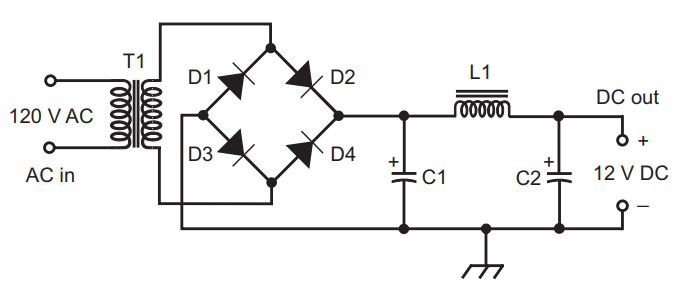
\includegraphics[width=\textwidth]{figuras/esquematico.png}
    \caption{Esquema elétrico do sistema.}
    \label{fig:esquema-eletrico}
\end{figure}



